\subsection{線形 Kalman フィルタから非線形ロボット運動学への接続}

相補フィルタは、ジャイロ積分の速い変化と、加速度計や他の低周波な測定から得る遅い補正を、あらかじめ決めた重みで混ぜる構成であった。姿勢だけを短時間でならす段階では有効であるが、差動二輪ロボットの走行では、重みを固定したままでは残るずれを扱いきれない。左車輪が一瞬すべったのか、ジャイロバイアスで向きが少しずれたのか、外部の位置測定が一時的に粗くなったのかによって、同じ位置ずれでも次に信じるべき信号は変わる。ここで必要になるのは、推定値そのものだけでなく、その推定値をどの方向にどの程度疑うかを表す共分散である。

前に導いた離散時間 Kalman フィルタは、この状況にそのまま使える二つの言葉を与えていた。第一に、モデルで進めた後の不確かさを予測共分散 $P^-$ として持つ。$P^-$ が大きい方向は、モデルだけでは推定が広がっている方向である。第二に、測定値と予測測定値の差を革新 $\nu$ と呼び、その革新をどれだけ状態へ戻すかを Kalman ゲイン $K$ で決める。測定ノイズが小さく、かつ $P^-$ が大きい方向を測っているなら、$K$ は大きくなる。測定が粗い、またはその測定では見えにくい方向なら、$K$ は小さくなる。この構造は、相補フィルタの固定重みを、現在の予測不確かさと測定不確かさに応じて変える仕組みとして読める。

ただし、線形 Kalman フィルタのままでは、差動二輪ロボットの姿勢を自然には進められない。ロボットの姿勢を
\begin{equation}
  X_k=
  \begin{bmatrix}
    x_k\\ y_k\\ \theta_k
  \end{bmatrix}
\end{equation}
とし、時刻 $k$ から $k+1$ までの左右車輪の移動量を $\Delta s_R,\Delta s_L$、車輪間隔を $b$ とする。短い区間の代表的な前進量と向きの変化を
\begin{equation}
  s_k=\frac{\Delta s_R+\Delta s_L}{2},
  \qquad
  \Delta\theta_k=\frac{\Delta s_R-\Delta s_L}{b}
\end{equation}
と置けば、最も単純な離散姿勢予測は
\begin{align}
  x_{k+1}&=x_k+s_k\cos\theta_k,\\
  y_{k+1}&=y_k+s_k\sin\theta_k,\\
  \theta_{k+1}&=\theta_k+\Delta\theta_k
  \label{eq:flow-six-pose-prediction}
\end{align}
である。前進量 $s_k$ はロボット本体の前方向に測った距離であるが、地図上の $x,y$ 成分に直すには現在の向き $\theta_k$ を使って回転しなければならない。そのため、状態遷移は $X_{k+1}=AX_k+Bu_k$ のような固定行列ではなく、$\sin\theta_k$ と $\cos\theta_k$ を含む非線形写像になる。実装では旋回中の離散化誤差を減らすために $\theta_k+\Delta\theta_k/2$ を使う中点式や、一定曲率を仮定した厳密な円弧式を使うことも多いが、いずれも向きから地図上の移動方向を作るため非線形である。

線形 Kalman フィルタの予測式をこの姿勢モデルへつなぐには、平均は非線形式そのもので進め、誤差だけを現在の推定値の近くで線形化する。記号を軽くするため、ここでは $s_k,\Delta\theta_k$ を既知のオドメトリ入力とみなし、写像
\begin{equation}
  f(X_k,u_k)=
  \begin{bmatrix}
    x_k+s_k\cos\theta_k\\
    y_k+s_k\sin\theta_k\\
    \theta_k+\Delta\theta_k
  \end{bmatrix}
\end{equation}
を使う。予測平均は
\begin{equation}
  \hat{X}_{k+1|k}=f(\hat{X}_{k|k},u_k)
\end{equation}
で進める。いま、真の姿勢が推定値から小さくずれて
\begin{equation}
  X_k=\hat{X}_{k|k}+\delta X_k,
  \qquad
  \delta X_k=
  \begin{bmatrix}
    \delta x_k\\ \delta y_k\\ \delta\theta_k
  \end{bmatrix}
\end{equation}
であるとする。$f$ を $\hat{X}_{k|k}$ のまわりで一次展開すると、
\begin{equation}
  \delta X_{k+1|k}\simeq F_k\delta X_k
\end{equation}
となり、状態に関するヤコビアンは
\begin{equation}
  F_k=
  \left.\frac{\pp f}{\pp X}\right|_{\hat{X}_{k|k},u_k}
  =
  \begin{bmatrix}
    1&0&-s_k\sin\hat{\theta}_{k|k}\\
    0&1& s_k\cos\hat{\theta}_{k|k}\\
    0&0&1
  \end{bmatrix}
  \label{eq:flow-six-pose-jacobian}
\end{equation}
である。オドメトリ入力にも不確かさを入れるなら、入力誤差を
\begin{equation}
  \delta u_k=
  \begin{bmatrix}
    \delta s_k\\ \delta(\Delta\theta_k)
  \end{bmatrix}
\end{equation}
と置き、
\begin{equation}
  G_k=
  \left.\frac{\pp f}{\pp u}\right|_{\hat{X}_{k|k},u_k}
  =
  \begin{bmatrix}
    \cos\hat{\theta}_{k|k}&0\\
    \sin\hat{\theta}_{k|k}&0\\
    0&1
  \end{bmatrix}
\end{equation}
も使う。入力誤差の共分散を $Q_{u,k}$ とすると、予測共分散は
\begin{equation}
  P_{k+1|k}
  =
  F_kP_{k|k}F_k^\T+G_kQ_{u,k}G_k^\T
  \label{eq:flow-six-pose-covariance-prediction}
\end{equation}
となる。これは線形 Kalman フィルタの $P^-=APA^\T+GQG^\T$ と同じ形であり、違いは固定行列 $A$ の代わりに、いまの姿勢と入力から計算した局所ヤコビアン $F_k$ を使う点にある。

\weq{flow-six-pose-jacobian} の第三列は、向きの不確かさが位置の不確かさへ変わる仕組みを直接表している。位置成分だけを抜き出すと
\begin{equation}
  \begin{bmatrix}
    \delta x_{k+1}\\
    \delta y_{k+1}
  \end{bmatrix}
  \simeq
  \begin{bmatrix}
    \delta x_k\\
    \delta y_k
  \end{bmatrix}
  +
  s_k
  \begin{bmatrix}
    -\sin\hat{\theta}_{k|k}\\
     \cos\hat{\theta}_{k|k}
  \end{bmatrix}
  \delta\theta_k
  +
  \begin{bmatrix}
    \cos\hat{\theta}_{k|k}\\
    \sin\hat{\theta}_{k|k}
  \end{bmatrix}
  \delta s_k
\end{equation}
である。$\delta s_k$ はロボットの進行方向に沿った誤差を作る。一方、$\delta\theta_k$ は進行方向に直交する向きの誤差を作り、その大きさはおおよそ $s_k\abs{\delta\theta_k}$ である。たとえば $\hat{\theta}_{k|k}=0$ で前進すれば、向き誤差は主に $y$ 方向の横ずれになる。したがって、同じ角度分散でも、短く動いた直後より長く進んだ後のほうが横方向の位置楕円は大きく伸びる。

この関係を共分散の成分で見ると、向き分散 $P_{\theta\theta}$ だけから位置平面へ入る寄与は
\begin{equation}
  s_k^2P_{\theta\theta}
  \begin{bmatrix}
    \sin^2\hat{\theta}_{k|k}&-\sin\hat{\theta}_{k|k}\cos\hat{\theta}_{k|k}\\
    -\sin\hat{\theta}_{k|k}\cos\hat{\theta}_{k|k}&\cos^2\hat{\theta}_{k|k}
  \end{bmatrix}
\end{equation}
の形になる。楕円が進行方向ではなく横方向へ広がるのは、この行列が
\begin{equation}
  \begin{bmatrix}
    -\sin\hat{\theta}_{k|k}\\
     \cos\hat{\theta}_{k|k}
  \end{bmatrix}
\end{equation}
方向の外積で作られているためである。角度を少し間違えたまま距離を進むと、地図上の終点が扇状にずれる。共分散楕円は、この扇状の広がりを推定値の近くで一つの楕円として近似したものである。

図\ref{fig:kalman-pose-bridge-examples} は、この接続を平面図で示している。左は差動二輪の平均姿勢を短いオドメトリ刻みで進めた軌跡であり、初期方位を $\pm\sigma_\theta$ だけ変えた破線と点線が、同じ車輪移動量でも終点が横へ分かれることを示す。中央は同じ予測に \weq{flow-six-pose-covariance-prediction} を繰り返し適用した $2\sigma$ 楕円であり、走行距離が増えるにつれて楕円が進行方向の法線側へ伸びる。右は一歩の局所幾何であり、前進ベクトル $s[\cos\theta,\sin\theta]^\T$ に対して、方位誤差の一次感度が $s[-\sin\theta,\cos\theta]^\T$ という接線方向の回転で表されることを示している。

\begin{figure}[tb]
\centering
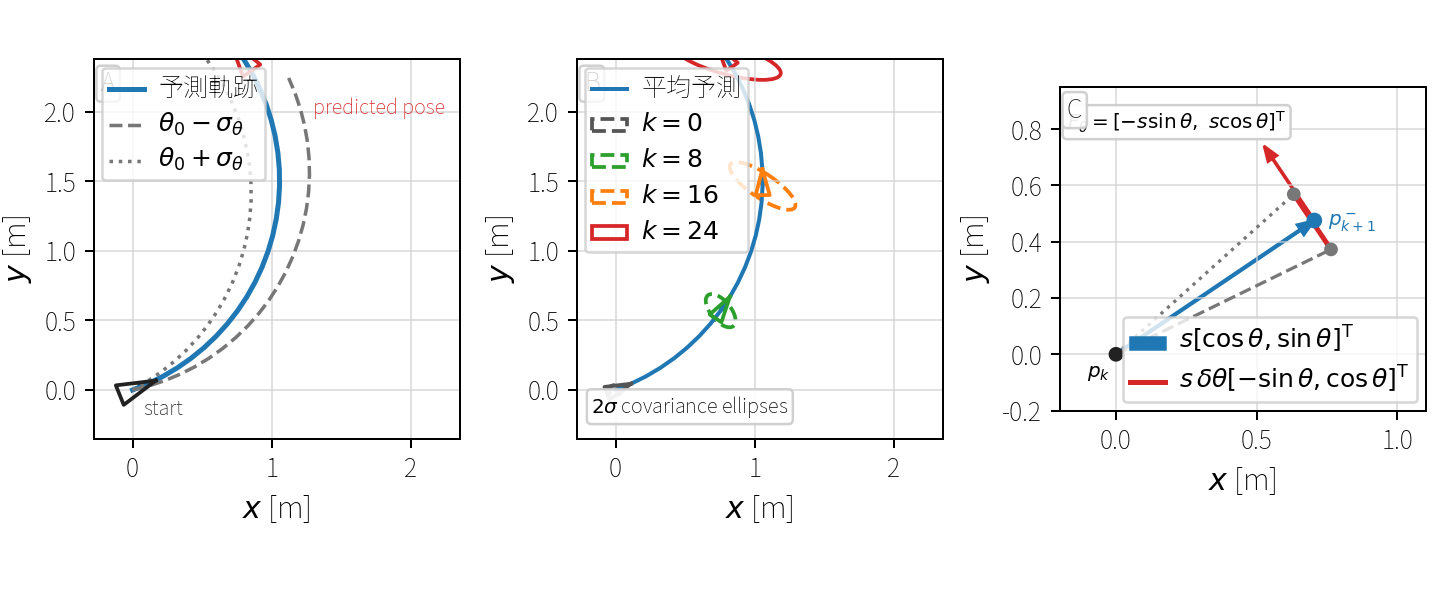
\includegraphics[width=0.96\linewidth,bb=0 0 1440 603]{figures/flow6_kalman_pose_bridge_examples.png}
\caption{線形 Kalman フィルタの共分散予測を差動二輪の非線形姿勢予測へ接続する幾何。左はオドメトリによる円弧状の平均姿勢予測と初期方位のずれによる終点差、中央は局所ヤコビアンで伝搬した $2\sigma$ 共分散楕円、右は $F_k$ の方位列が前進距離に比例した横方向感度を表すことを示している。}
\label{fig:kalman-pose-bridge-examples}
\end{figure}

ここまでで、相補フィルタの固定重みでは扱いにくかったセンサ融合の失敗は、$P^-$、革新、Kalman ゲインという線形 Kalman フィルタの二段構造で読み替えられることが分かる。同時に、ロボットの姿勢予測そのものは $\sin\theta$ と $\cos\theta$ を含むため、固定行列の線形モデルには戻らない。残る手順は、時々刻々の予測点で $F_k$ を作り、測定式も必要なら同じように局所線形化して、線形 Kalman フィルタの予測と更新の形へ入れることである。この手順が、次に扱う拡張 Kalman フィルタの出発点になる。
